\documentclass[12pt,a4paper,oneside]{report} %<<<1 ------------------------------
% fonts, encoding:
\usepackage[utf8]{inputenc}             % file is in utf8:
\usepackage{cmap}                       % pdf is created with correct special characters, requires proper font, see next two lines
\usepackage[T1]{fontenc}                % see higher line
\usepackage{tgtermes}                   % high quality times font
\usepackage{textcomp}                   % proper micro sign for SI, use: \textmu, in equation: $\hbox{\textmu}$
\usepackage{slantsc}                   % proper micro sign for SI, use: \textmu, in equation: $\hbox{\textmu}$
\usepackage{calc}                   % provides \widthof
\usepackage{enumitem}                   % provides \begin{description} with settings []
\usepackage{color}                   % provides coloured text
% obrazky:
\usepackage{graphicx}                   % to insert pictures
\usepackage{grffile}                    % enables spaces in picture file names
\grffilesetup{ multidot=false, babel=false, encoding, inputencoding=utf8, filenameencoding=utf8, space=true}
\newcommand*{\FILEDOT}{.}                   % if picture file name containt dot (e.g. aaa.bbb.pdf), then TeX considers rest as filename extension, so dot must be written as follows: \includegraphics{aaa\FILEDOT bbb.eps}
% rest:
\usepackage[pdftex,
            unicode,
            pdfauthor={Q-Wave consorcium},
            pdftitle={Quantum Wave ToolBox documentation},
            pdfkeywords={algorithm, data procesing, sampling, toolbox},
            pdfproducer={Latex with hyperref},
            pdfcreator={pdflatex}]{hyperref}
%\usepackage[a4paper]{geometry}          % ensure A4
%\geometry{verbose,lmargin=2.5cm,rmargin=2.5cm,tmargin=2.5cm,bmargin=2.5cm}      % margins settings
\usepackage{url}                        % enables \url in bibtex
%\usepackage{setspace} \doublespacing   % double line spacing, for 1.5 set \onehalfspace
\usepackage{xspace}                     % proper automatic spacing after user defined commands
\usepackage{amsmath}                    % better equations

% lstlisting settings %<<<1 ----------------------------------------------------
\usepackage{listings}                   % for source code formatting
\definecolor{mygreen}{rgb}{0,0.6,0}
\definecolor{mygray}{rgb}{0.5,0.5,0.5}
\definecolor{lightgray}{rgb}{0.95,0.95,0.95}
\definecolor{mymauve}{rgb}{0.58,0,0.82}

\lstdefinestyle{mcode}{
%\lstset{ %
  backgroundcolor=\color{lightgray},   % choose the background color; you must add \usepackage{color} or \usepackage{xcolor}
  basicstyle=\normalsize\sffamily,        % the size of the fonts that are used for the code
  breakatwhitespace=false,         % sets if automatic breaks should only happen at whitespace
  breaklines=true,                 % sets automatic line breaking
  captionpos=b,                    % sets the caption-position to bottom
  commentstyle=\color{mygreen},    % comment style
  deletekeywords={...},            % if you want to delete keywords from the given language
  escapeinside={\%*}{*)},          % if you want to add LaTeX within your code
  extendedchars=true,              % lets you use non-ASCII characters; for 8-bits encodings only, does not work with UTF-8
  frame=single,	                   % adds a frame around the code
  keepspaces=true,                 % keeps spaces in text, useful for keeping indentation of code (possibly needs columns=flexible)
  keywordstyle=\color{blue},       % keyword style
  language=Matlab,                 % the language of the code
  otherkeywords={*,qwtb,alg_info,alg_wrapper,
        normrnd, alg_test,alg_example,...},           % if you want to add more keywords to the set
  numbers=none,                    % where to put the line-numbers; possible values are (none, left, right)
  numbersep=5pt,                   % how far the line-numbers are from the code
  numberstyle=\tiny\color{mygray}, % the style that is used for the line-numbers
  rulecolor=\color{black},         % if not set, the frame-color may be changed on line-breaks within not-black text (e.g. comments (green here))
  showspaces=false,                % show spaces everywhere adding particular underscores; it overrides 'showstringspaces'
  showstringspaces=false,          % underline spaces within strings only
  showtabs=false,                  % show tabs within strings adding particular underscores
  stepnumber=2,                    % the step between two line-numbers. If it's 1, each line will be numbered
  stringstyle=\color{mymauve},     % string literal style
  tabsize=2,                       % sets default tabsize to 2 spaces
  title=\lstname,                  % show the filename of files included with \lstinputlisting; also try caption instead of title
  belowskip=0pt                  % skip after end of lstlistings
}

\lstdefinestyle{output}{
%\lstset{ %
  backgroundcolor=\color{lightgray},   % choose the background color; you must add \usepackage{color} or \usepackage{xcolor}
  basicstyle=\normalsize\itshape,        % the size of the fonts that are used for the code
  breakatwhitespace=false,         % sets if automatic breaks should only happen at whitespace
  breaklines=true,                 % sets automatic line breaking
  captionpos=b,                    % sets the caption-position to bottom
  commentstyle=\color{mygreen},    % comment style
  deletekeywords={...},            % if you want to delete keywords from the given language
  escapeinside={\%*}{*)},          % if you want to add LaTeX within your code
  extendedchars=true,              % lets you use non-ASCII characters; for 8-bits encodings only, does not work with UTF-8
  frame=none,	                   % adds a frame around the code
  keepspaces=true,                 % keeps spaces in text, useful for keeping indentation of code (possibly needs columns=flexible)
  keywordstyle=\color{blue},       % keyword style
  language=Matlab,                 % the language of the code
  otherkeywords={*,qwtb,alg_info,alg_wrapper,alg_test,alg_example,...},           % if you want to add more keywords to the set
  numbers=none,                    % where to put the line-numbers; possible values are (none, left, right)
  numbersep=5pt,                   % how far the line-numbers are from the code
  numberstyle=\tiny\color{mygray}, % the style that is used for the line-numbers
  rulecolor=\color{black},         % if not set, the frame-color may be changed on line-breaks within not-black text (e.g. comments (green here))
  showspaces=false,                % show spaces everywhere adding particular underscores; it overrides 'showstringspaces'
  showstringspaces=false,          % underline spaces within strings only
  showtabs=false,                  % show tabs within strings adding particular underscores
  stepnumber=2,                    % the step between two line-numbers. If it's 1, each line will be numbered
  stringstyle=\color{mymauve},     % string literal style
  tabsize=2,                       % sets default tabsize to 2 spaces
  title=\lstname,                  % show the filename of files included with \lstinputlisting; also try caption instead of title
  belowskip=0pt,                  % skip after end of lstlistings
  xleftmargin=20pt                      % margin on left side
}

\lstset{style=mcode}
     % user defined code formatting

% bibliography settings %<<<1 ----------------------------------------------------
\usepackage[english]{babel} % main language of the document must be last
\usepackage[
   backend=biber      % if we want unicode 
  ,style=ieee   % or iso-numeric for numeric citation method          
  ,babel=other        % to support multiple languages in bibliography
  %,sortlocale=cs_CZ   % locale of main language, it is for sorting
  ,sortlocale=en_UK   % locale of main language, it is for sorting
  ,bibencoding=UTF8   % this is necessary only if bibliography file is in different encoding than main document
]{biblatex}

\bibliography{alllib2}
%\defbibenvironment{bibliography}
%    {\list
%        {[\printfield[labelnumberwidth]{labelnumber}]}
%        {\setlength{\labelwidth}{\labelnumberwidth}
%        \setlength{\leftmargin}{4pt}
%        \setlength{\labelsep}{10pt}
%        \addtolength{\leftmargin}{\labelsep}
%        \setlength{\itemsep}{6pt}
%        \setlength{\parsep}{\bibparsep}}
%        \renewcommand*{\makelabel}[1]{\hss##1}}
%    {\endlist}
%    {\item}

% shorts: %<<<1 ----------------------------------------------------

\def\Alg{{\sc Algorithm}\xspace}
\def\Algs{{\sc Algorithms}\xspace}
\def\Tb{{\sc Toolbox}\xspace}
\def\Da{{\sc Data}\xspace}
\def\Mea{{\sc Measurement}\xspace}
\def\Qua{{\sc Quantity}\xspace}
\def\Quas{{\sc Quantities}\xspace}
\def\Wr{{\sc Wrapper}\xspace}
\def\Wrs{{\sc Wrappers}\xspace}
\def\matlab{{\sc MATLAB}\xspace}
\def\octave{{\sc GNU Octave}\xspace}
\def\labview{{\sc LabVIEW}\xspace}
\def\mgo{\matlab/\octave\xspace}
        
\begin{document} % other document settings --------------------------------------------%<<<1
% how to devide special words, e.g. auto-mation
\hyphenation{Frame-work OpenOffice SourceForge Windows}
%\def\thesection{\Roman{section}}       % redefines numbering style of sections
\renewcommand\floatpagefraction{.9} \renewcommand\topfraction{.9} \renewcommand\bottomfraction{.9} \renewcommand\textfraction{.1} \setcounter{totalnumber}{50} \setcounter{topnumber}{50} \setcounter{bottomnumber}{50} % if too many pictures, change text/float fraction
\renewcommand{\labelitemi}{--}          % item sepparator
\setlength{\unitlength}{1mm}            % default length in picture environment

% tight description environment:
\newenvironment{tightdesc}{\begin{description}[itemsep=0pt]} 
                              {\end{description}}

% names of sections:
\def\infosection{Description}
\def\examplesection{Example}
% remove "chapter" from chapter heading:
\renewcommand{\chaptername}{}

\title{Quantum Wave ToolBox: Toolbox description}
\author{Q-Wave consorcium}

% first page ----------------------------------------------------------------------- %<<<1 ------------------------------
\thispagestyle{empty}
\begin{center}
        \vspace*{10em}
        {\huge
        
\includegraphics[width=0.3\textwidth]{logo/qwtb_logo.pdf}

        \vspace{0.5em}
        Quantum Wave ToolBox\\

        \vspace{1.5em}
        Toolbox description}\\

        \vfill
        {\Large \color{red}{QWTB version 0.1}}

        \vspace{1em}
        {\Large \url{https://qwtb.github.io/qwtb/}}
\end{center}
\newpage

\tableofcontents

\chapter{Introduction} %<<<1 ------------------------------
\bigskip
\begin{center}
        \parbox{0.7\textwidth}{\textit{Press a button with bold title AMPLITUDE\\
        \dots drink a coffee \dots\\
        and get the result}}
\end{center}

\bigskip
\noindent Quantum Wave ToolBox (QWTB) is a toolbox for evaluation of measured data. QWTB consist of data
processing algorithms from very different sources and unificating application interface. The toolbox
gives the possibility to use different data processing algorithms with one set of data and removes
the need to reformat data for every particular algorithm. Toolbox is extensible. The toolbox
can variate input data and calculate uncertainties by means of Monte Carlo Method
(MCM)~\cite{JCGM2008}.

Toolbox was realized within the EMRP-Project SIB59 Q-Wave. The EMRP is jointly funded by the EMRP
par- ticipating countries within EURAMET and the European Union.

\vfill

\includegraphics[width=0.3\textwidth]{sources/Q-Wave_logo_01.pdf}
\hfill

\includegraphics[width=0.3\textwidth]{sources/eurametlogo.jpg}


\chapter{Basic description of the toolbox} %<<<1 ------------------------
\section{Toolbox overall scheme} %<<<2 ------------------------------
The basic scheme of the toolbox is following:
\begin{center}
        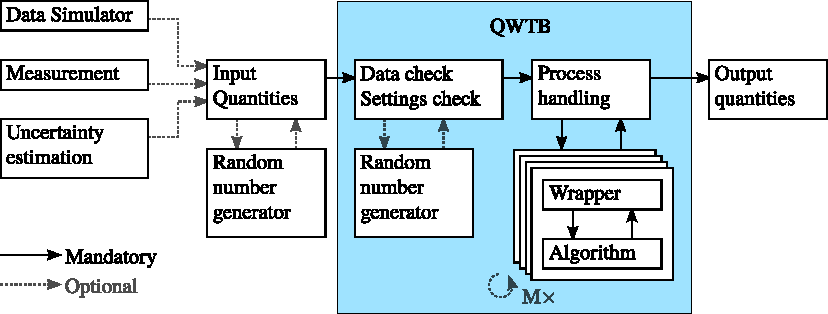
\includegraphics{sources/basic scheme v2.pdf}
\end{center}

User have to prepare the data, either based on a real measurement or simulated, into a specified
format. If needed, user can generate randomized data for selected quantities (e.g. with special
probability density functions) and prepare for Monte Carlo uncertainty calculation. Next user calls
toolbox to apply a selected algorithm on the data and review results. Toolbox will:
\begin{enumerate}
        \item Check user data.
        \item Check or generate calculation settings.
        \item If required, quantities are randomized according uncertainties to prepare for MCM uncertainty calculation.
        \item Data are handled to a wrapper. If needed, wrapper is run multiple times according MCM.
        \item Output data are the result of the toolbox.
\end{enumerate}

Another algorithm can be used immediately on the same data. User interface of the toolbox is represented
by the function \lstinline{qwtb} defined in the file {\tt qwtb.m}.

\section{Toolbox use} %<<<2 ------------------------------
The toolbox is used in several modes according to a number and character of input arguments.

\subsection{Get list of implemented algorithms} %<<<3
\begin{lstlisting}
alginfo = qwtb()
\end{lstlisting}

With no input arguments, toolbox returns informations on all available algorithms. Result array
\lstinline{alginfo} contains structures for every algorithm found in the same directory as
\texttt{qwtb.m}. Format of structures is defined in~\ref{structalginfo}.

\subsection{Application of an algorithm on the data} %<<<3 ------------------------------
\begin{lstlisting}
dataout = qwtb('algid', datain)
\end{lstlisting}

The algorithm is selected by first input argument \lstinline{algid}. It is a string with
designator of the algorithm, according structrue~\ref{structalginfo}.

The second input argument is the user data. Data have to be formatted in a structure with fields
named as quantities required by the algorithm (see~\ref{structquantity}).

The output variable is the structure with fields named as quantities.

In this case, standard calculation settings are used. If the user specifies calculation settings
in structure according~\ref{structcalcset}, it can be used as third input argument
\lstinline{calcset}:

\begin{lstlisting}
dataout = qwtb('algid', datain, calcset)
\end{lstlisting}

For some calculation settings some fields of \lstinline{datain} or \lstinline{calcset} are generated
automatically. To review automatically generated fields, user can get these structure in second and
third output argument:

\begin{lstlisting}
[dataout, datain, calcset] = qwtb('algid', datain)
[dataout, datain, calcset] = qwtb('algid', datain, calcset)
\end{lstlisting}

\subsection{Running an example of algorithm use} %<<<3 ------------------------------
Algorithm can have implemented an example of the use. This can be run by following syntax:

\begin{lstlisting}
qwtb('algid', 'example')
\end{lstlisting}

The algorithm is selected by first input argument \lstinline{algid}. It is a string with
designator of the algorithm, according structrue~\ref{structalginfo}. The second argument is a
string. Toolbox will run a script \lstinline{alg_example.m} located in a algorithm directory.

After finish user can review input and output data or resulted figures if any.

\subsection{Running a test of algorithm} %<<<3 ------------------------------
Algorithm can have implemented a self test. This can be run by following syntax:

\begin{lstlisting}
qwtb('algid', 'test')
\end{lstlisting}

The algorithm is selected by first input argument \lstinline{algid}. It is a string with
designator of the algorithm, according structrue~\ref{structalginfo}. The second argument is a
string. Toolbox will run a script \lstinline{alg_test.m} located in a algorithm directory.

Test should prepare data, run algorithm and check results. If implementation of algorithm
behaves incorrectly, an error will occur.

\subsection{Adding or removing algorithm path} %<<<3 ------------------------------
Algorithms are stored in different directories, which are not in \mgo load path. To add directory
with selected path to \mgo load path, following syntax is used:

\begin{lstlisting}
qwtb('algid', 'addpath')
\end{lstlisting}

To remove path, use:

\begin{lstlisting}
qwtb('algid', 'rempath')
\end{lstlisting}

Adding or removing path should be required only in special cases, such as debugging etc.

\subsection{Displaying license of an algorithm} %<<<3 ------------------------------------
To display a license of an algorithm, following syntax is used:
\begin{lstlisting}
license = qwtb('algid', 'license')
\end{lstlisting}
For details on licensing, see chapter~\ref{ch-license}.


\chapter{Detailed description of the toolbox} %<<<1 ------------------------------
\section{Algorithm directory structure implementation} %<<<2 ------------------------------
\label{diralg}
Every algorithm is placed in a directory of following name:
\begin{center}
        {\tt alg\_X}
\end{center}
These directories have to be located in the directory containing the toolbox main script {\tt qwtb.m}.

Every algorithm directory contains following files:
\begin{tightdesc}
        \item [{\tt X1}, {\tt X2}, \dots] ---  Mandatory. One or more files with the algorithm itself.
        \item [{\tt alg\_info.m}] ---  Mandatory. Description of the algorithm. See \ref{filealginfo}.
        \item [{\tt alg\_wrapper.m}] ---  Mandatory. Wrapper of the algorithm. See \ref{filealgwrapper}.
        \item [{\tt alg\_test.m}] ---  Recomended. Testing function. See \ref{filealgtest}.
        \item [{\tt alg\_example.m}] ---  Recomended. Example script. See \ref{filealgexample}.
\end{tightdesc}

\subsection{File {\tt alg\_info.m}} %<<<3 ------------------------------
\label{filealginfo}
File contains a function with definition:

\begin{lstlisting}
function alginfo = alg_info()
\end{lstlisting}

The output \lstinline{alginfo} is a structure with informations about the algorithm. Structure is
defined in~\ref{structalginfo}.

File is mandatory. If file is missing in algorithm directory, QWTB will not recognize this
algorithm as part of the toolbox.

\subsection{File {\tt alg\_wrapper.m}} %<<<3 ------------------------------
\label{filealgwrapper}
File contains a function with definition:

\begin{lstlisting}
function dataout = alg_wrapper(datain, calcset)
\end{lstlisting}

The input \lstinline{datain} is a structure with input data (see %XXX
), \lstinline{calcset} is a structure with definition of calculation settings
(see~\ref{structcalcset}).
) and \lstinline{dataout} is a structure containing output data (see %XXX
).

The wrapper does following:
\begin{enumerate}
        \item Formats input data structure \lstinline{datain} into variables wuitable for algorithm.
        \item Runs the algorithm.
        \item Format results of the algorithm into data structure \lstinline{dataout}.
\end{enumerate}

File is mandatory. If file is missing in algorithm directory, QWTB will not recognize this
algorithm as part of the toolbox.

\subsection{File {\tt alg\_test.m}} %<<<3 ------------------------------
\label{filealgtest}
File contains a function with following definition:

\begin{lstlisting}
function alg_test(calcset)
\end{lstlisting}

Test should generate sample data, run algorithm and check results by a function \lstinline{assert}.
QWTB will provide a standard calculation settings structure \lstinline{calcset} (see~\ref{structcalcset}).

This file is not mandatory, however is recommended.

\subsection{File {\tt alg\_example.m}} %<<<3 ------------------------------
\label{filealgexample}

Example contains a script showing a basic use of the algorithm. The format of the file should
conform to the publishing markup defined in Matlab documentation. See matlab help on keyword
\emph{Publishing markup}). The QWTB runs this script in base context, thus all variables defined in
the example script will be accessible to the user.

To create a documentation of the QWTB, function \lstinline{publish} is applied to the example script
and resulting file is attached to the documentation file.

\section{Algorithm informations structure} %<<<2 ------------------------------
\label{structalginfo}
Structure defines properties and possibilities of the algorithm. All fields are mandatory but
\lstinline{.fullpath}.

\begin{tightdesc}
        \item [\textsf{.id}] --- Designator of the algorithm.
        \item [\textsf{.name}] ---  Name of the algorithm.
        \item [\textsf{.desc}] ---  Basic description.
        \item [\textsf{.citation}] ---  Reference.
        \item [\textsf{.remarks}] ---  Any remark.
        \item [\textsf{.license}] ---  License of the algorithm.
        \item [\textsf{.requires}] ---  Required quantities.
        \item [\textsf{.reqdesc}] ---  Short description of required quantities.
        \item [\textsf{.returns}] ---  Output quantities.
        \item [\textsf{.retdesc}] ---  Short description of output quantities.
        \item [\textsf{.providesGUF}] ---  Algorithm/wrapper calculates GUF uncertainty.
        \item [\textsf{.providesMCM}] ---  Algorithm/wrapper calculates MCM uncertainty.
        \item [\textsf{.fullpath}] ---  Full path to the algorithm. Automatically generated by the toolbox.
\end{tightdesc}

\subsection{\textsf{.id}} %<<<3 ------------------------------
String. Designator of the algorithm. It is unique identifier, no two algorithms can have same id.

\subsection{\textsf{.longname}} %<<<3 ------------------------------
String. Full name of the algorithm. 

\subsection{\textsf{.desc}} %<<<3 ------------------------------
String. Basic description of the algorithm.

\subsection{\textsf{.citation}} %<<<3 ------------------------------
String. A reference to the paper, book or other literature with full description of the algorithm.

\subsection{\textsf{.remarks}} %<<<3 ------------------------------
String. Remarks or others related to the algorithm.

\subsection{\textsf{.license}} %<<<3 ------------------------------
String. License of the algorithm. This is not license of the toolbox but of the algorithm!

\subsection{\textsf{.requires}} %<<<3 ------------------------------
Cell array of strings. Names of quantities required by the algorithm.

\subsection{\textsf{.reqdesc}} %<<<3 ------------------------------
Cell array of strings. Short description of quantities required by the algorithm.

\subsection{\textsf{.returns}} %<<<3 ------------------------------
Cell array of strings. Names of quantities returned by the algorithm.

\subsection{\textsf{.retdesc}} %<<<3 ------------------------------
Cell array of strings. Short description of quantities returned by the algorithm.

\subsection{\textsf{.providesGUF}} %<<<3 ------------------------------
Boolean. If nonzero, the wrapper or the algorithm calculates uncertainty by means of GUM Uncertainty
Framework.

\subsection{\textsf{.providesMCM}} %<<<3 ------------------------------
Boolean. If nonzero, the wrapper or the algorithm calculates uncertainty by means of Monte Carlo
Method.

\subsection{\textsf{.fullpath}} %<<<3 ------------------------------
String. Full path to the algorithm. This field is automatically generated by QWTB.

\section{Quantity structure} %<<<2 ------------------------------
\label{structquantity}
Every quantity is a structure with following fields:
\begin{tightdesc}
        \item [\textsf{.v}] --- Value.
        \item [\textsf{.u}] --- Uncertainty.
        \item [\textsf{.d}] --- Degree of freedom.
        \item [\textsf{.c}] --- Correlation.
        \item [\textsf{.r}] --- Randomized uncertainty.
\end{tightdesc}

\subsection{\textsf{.v}} %<<<3 ------------------------------
Value of the quantity. Can be a scalar, \emph{row} vector or matrix. More dimensions are not supported.

\subsection{\textsf{.u}} %<<<3 ------------------------------
Standard uncertainty of the quantity. Dimensions are the same as of the value field. 

\subsection{\textsf{.d}} %<<<3 ------------------------------
Degrees of freedom the uncertainty according GUM Uncertainty Framework. Dimensions are the same as of the value field.

This field is automatically generated by the toolbox if missing, required and \lstinline{calcset.dof.gen}
is set to nonzero. The value will be set to 50.

\subsection{\textsf{.c}} %<<<3 ------------------------------
Correlation matrix for quantity. 2DO XXX.

This field can be automatically generated by the toolbox if missing, required and \lstinline{calcset.cor.gen}
is set to nonzero. The value will be set to 0.

\subsection{\textsf{.r}} %<<<3 ------------------------------
Randomized uncertainties according Monte Carlo method. In the case of scalar quantity it is
\emph{column} vector of length equal to \lstinline{calcset.mcm.repeats}. For a vector quantity it is a matrix with number
of columns equal to length of value of the quantity and number of rows equal to
\lstinline{calcset.mcm.repeats}. For a matrix quantity it is a matrix with three dimensions, first
two equal to the dimensions of value quantity, third dimension equal to
\lstinline{calcset.mcm.repeats}.

This field is required if Monte Carlo uncertainty calculation is required. In this case it can be
automatically generated by the toolbox if missing and \lstinline{calcset.mcm.randomize} is set to
boolean. The pdf will be normal, sigma will be equal to the standard uncertainty of the quantity.

\subsection{Quantity structure examples} %<<<3 ------------------------------
Example of scalar quantity of mean value 1, standard uncertainty 0.1, degrees of freedom 9, correlation has no
sense for scalar quantity, and radnomized matrix has number of elements equal to \lstinline{calcset.mcm.randomize}.
\begin{eqnarray*}
        \text{\textsf{.v}:} &(1)\\
        \text{\textsf{.u}:} &(0.1)\\
        \text{\textsf{.d}:} &(9)\\
        \text{\textsf{.c}:} &(0)\\
        \text{\textsf{.r}:} &\begin{pmatrix}
                1.02076 \\
                1.22555 \\
                \vdots\\
                0.89727 \\
        \end{pmatrix}\\
\end{eqnarray*}

Example of vector quantity with $i$ elements, $M$ is equal to \lstinline{calcset.mcm.randomize} (only symbolic representation):
\begin{eqnarray*}
        \text{\textsf{.v}:} & (v_1, v_2, \dots, v_i) \\
        \text{\textsf{.u}:} & (u_1, u_2, \dots, u_i) \\
        \text{\textsf{.d}:} & (d_1, d_2, \dots, d_i) \\
        \text{\textsf{.c}:} & \left(    \begin{array}{ccc}
                                                c_{11}  & \hdots & c_{1i} \\
                                                \vdots  & \ddots & \vdots \\
                                                c_{i1}  & \hdots & c_{ii} \\
                                        \end{array}\right) \\
        \text{\textsf{.r}:} & \left(    \begin{array}{ccc}
                                                r_{11}  & \hdots & r_{1i} \\
                                                \vdots  & \ddots & \vdots \\
                                                r_{M1}  & \hdots & r_{Mi} \\
                                        \end{array}\right) \\
\end{eqnarray*}

Example of matrix quantity with $i$ times $j$ elements, $M$ is equal to \lstinline{calcset.mcm.randomize} (only symbolic representation):
\begin{eqnarray*}
        \text{\textsf{.v}:} & \left(    \begin{array}{ccc}
                                                v_{11}  & \hdots & v_{1j} \\
                                                \vdots  & \ddots & \vdots \\
                                                v_{i1}  & \hdots & v_{ij} \\
                                        \end{array}\right) \\
        \text{\textsf{.u}:} & \left(    \begin{array}{ccc}
                                                v_{11}  & \hdots & u_{1j} \\
                                                \vdots  & \ddots & \vdots \\
                                                u_{i1}  & \hdots & u_{ij} \\
                                        \end{array}\right) \\
        \text{\textsf{.d}:} & \left(    \begin{array}{ccc}
                                                d_{11}  & \hdots & d_{1j} \\
                                                \vdots  & \ddots & \vdots \\
                                                d_{i1}  & \hdots & d_{ij} \\
                                        \end{array}\right) \\
        \text{\textsf{.c}:} & \left(    XXX??? \right) \\
        \text{\textsf{.r}:} & \left(    \begin{array}{ccc}
                                                r_{111}  & \hdots & r_{1j1} \\
                                                \vdots  & \ddots & \vdots \\
                                                r_{i11}  & \hdots & r_{ij1} \\
                                        \end{array}\right) \\
                            & \qquad\vdots                        \\
                            & \left(    \begin{array}{ccc}
                                                r_{11M}  & \hdots & r_{1jM} \\
                                                \vdots  & \ddots & \vdots \\
                                                r_{i1M}  & \hdots & r_{ijM} \\
                                        \end{array}\right) \\
\end{eqnarray*}

\section{Calculation settings structure} %<<<2 ------------------------------
\label{structcalcset}
Structure defines calculation methods.
\begin{tightdesc}
        \item [\textsf{.strict}] ---  (0) If zero, other fields generated automatically.
        \item [\textsf{.verbose}] ---  (1) Display various informations.
        \item [\textsf{.unc}] ---  ('none') How uncertainty is calculated ('none', 'guf', 'mcm').
        \item [\textsf{.cor.req}] ---  (0) Correlation matrix is required for all input quantities.
        \item [\textsf{.cor.gen}] ---  (1) Zero correlation matrix is generated automatically if missing.
        \item [\textsf{.dof.req}] ---  (1) Degrees of freedom are required for all input quantities.
        \item [\textsf{.dof.gen}] ---  (1) Degree of freedom are generated automatically if missing with value 50.
        \item [\textsf{.mcm.repeats}] ---  (100) Number of Monte Carlo iterations.
        \item [\textsf{.mcm.verbose}] ---  (1) Display various informations concerning Monte Carlo method.
        \item [\textsf{.mcm.method}] ---  ('singlecore') Parallelization method ('multicore', 'multistation').
        \item [\textsf{.mcm.procno}] ---  (1) Number of processors to use.
        \item [\textsf{.mcm.tmpdir}] ---  ('.') Directory for temporary data.
        \item [\textsf{.mcm.randomize}] ---  (1) Randomized uncertainties are generated automatically if missing.
\end{tightdesc}

\subsection{\textsf{.strict}} %<<<3 ------------------------------
Boolean, default value 0. If set to zero, all other fields of the structure are generated
automatically and set to a default value.

\subsection{\textsf{.verbose}} %<<<3 ------------------------------
Boolean, default value 1. If set to non-zero value, various messages are displayed during
calculation, such as used uncertainty calculation method, automatic generation of matrices etc.

\subsection{\textsf{.unc}} %<<<3 ------------------------------
String, default value ''. Determines uncertainty calculation method. Only three values are possible:
\begin{tightdesc}
        \item [\textsf{''}] ---  Uncertainty is not calculated.
        \item [\textsf{'guf'}] ---  Uncertainty is calculated by GUM Uncertainty Framework~\cite{JCGM1995}.
        \item [\textsf{'mcm'}] ---  Uncertainty is calculated by Monte Carlo Method~\cite{JCGM2008}.
\end{tightdesc}
See chapter XXX %XXX
for uncertainty calculation details.

\subsection{\textsf{.cor}} %<<<3 ------------------------------
Structure sets handling of correlation matrices of quantities. Structure has two fields:
\begin{tightdesc}
        \item [\textsf{.req}] ---  Boolean, default value 0. If non-zero, correlation matrices are required for all quantities.
        \item [\textsf{.gen}] ---  Boolean, default value 1. If non-zero, correlation matrices will be generated
        automatically if missing in quantity.
\end{tightdesc}
Automatically generated correlation matrices has all elements of zero value.

\subsection{\textsf{.dof}} %<<<3 ------------------------------
Structure sets handling of degrees of freedom of quantities. Structure has two fields:
\begin{tightdesc}
        \item [\textsf{.req}] ---  Boolean, default value 0. If non-zero, degrees of freedom are required for all quantities.
        \item [\textsf{.gen}] ---  Boolean, default value 1. If non-zero, degree of freedom will be generated
        automatically if missing in quantity.
\end{tightdesc}
Automatically generated degree of freedom has value 50.

\subsection{\textsf{.mcm}} %<<<3 ------------------------------
Structure sets handling of Monte Carlo calculation of uncertainties. Structure has following fields:
\begin{tightdesc}
        \item [\textsf{.repeats}] ---  Positive non-zero integer, default value 100. Number of iterations of Monte Carlo method.

        \item [\textsf{.verbose}] ---  Boolean, default value 1. If set to non-zero value, various messages
        are displayed during calculation of Monte Carlo method such as used parallelization method,
        number of calculated iterations etc.

        \item [\textsf{.method}] ---  String, default value 'singlecore'. Parallelization method used for Monte
        Carlo method calculation. Only three values are possible:
        \begin{tightdesc}
                \item [\textsf{'singlecore'}] ---  No parallelization, all is calculated on one CPU core.
                \item [\textsf{'multicore'}] ---  Calculation is divided into cores of one computer.
                \item [\textsf{'multistation'}] ---  Calculation is distributed on several computers.
        \end{tightdesc}
        Not all methods are possible to use on all computers. 'singlecore' is always possible to
        use. 'multicore' use parfor in Matlab or parcellfun in GNU Octave. 'multistation' use %XXX

        \item [\textsf{.procno}] ---  Zero or positive integer, default value 0. Number of CPU cores exploitable
        by the parallelization method \textsf{'multicore'}. If set to zero, all available CPU cores will be used. If
        desktop computer is used, it is good practice to set to number of CPU cores minus one, so
        the computer can be used by other task also. 
        Works only in \octave.

        \item [\textsf{.tmpdir}] ---  String, default value '.' (current directory). Temporary directory for
        storing temporary data needed for some parallelization methods. %XXX which ones?

        \item [\textsf{.randomize}] ---  Boolean, default value 1. If non-zero, randomized uncertainties will be
        generated automatically if missing, but only if uncertainty calculation method is set to
        'mcm' (Monte Carlo) to prevent large memory usage.
\end{tightdesc}

\section{How uncertainty calculation works} %<<<2 ----------------------------------------
%2DO

\section{How to add a new algorithm} %<<<2 ----------------------------------------
%2DO
To add a new algorithm, several steps have to be done.

\begin{enumerate}
        \item Select an algorithm ID. Usually it is an acronym or abbreviation of the new algorithm name.

        \item Create a directory named {\tt alg\_SOMEID}, where {\tt SOMEID} is a selected ID. For a
        directory structure, see~\ref{diralg}.

        \item Put all files required by the algorithm (i.e. scripts, libraries) into the directory
        {\tt alg\_SOMEID/}.

        \item Create a file {\tt alg\_SOMEID/alg\_info.m}. An example of such file follows.
        \begin{lstlisting}
        function info = alg_info() %<<<1
        % Part of QWTB. Info script for algorithm SOMEALG.
        %
        % See also qwtb

        info.id = 'SOMEID';
        info.name = 'SOMEALG';
        info.desc = 'SOMEID is an super mega hyper algorithm for calculation of the ultimate answer to everything.';
        info.citation = 'Some nifty paper in some super journal.';
        info.remarks = 'Very simple implementation';
        info.license = 'MIT License';
        info.requires = {'a', 'b'};
        info.reqdesc = {'some input', 'some more important input'};
        info.returns = {'x', 'y', 'z'};
        info.retdesc = {'some output', 'some more important output', 'other output};
        info.providesGUF = 1;
        info.providesMCM = 0;
        \end{lstlisting}

        \item Create a wrapper for the algorithm in a file {\tt alg\_SOMEID/alg\_wrapper.m}, see~\ref{filealgwrapper}. An example of simple wrapper
        file follows.
        \begin{lstlisting}
        function dataout = alg_wrapper(datain, calcset)
        % Part of QWTB. Wrapper script for algorithm SOMEALG.
        %
        % See also qwtb

        % Format input data --------------------------- %<<<1
        % SOMEALG definition is:
        % function [x, y, z] = SOMEALG(a, b);
        a = datain.a.v;
        b = datain.b.v;

        % Call algorithm ---------------------------  %<<<1
        [x, y, z] = SOMEALG(a, b);

        % Format output data:  --------------------------- %<<<1
        dataout.x.v = x;
        dataout.y.v = y;
        dataout.z.v = z;

        end % function
        \end{lstlisting}

        \item Put a license of the algorithm into the file {\tt alg\_SOMEID/LICENSE.txt}.

        \item Create a testing script {\tt alg\_SOMEID/alg\_test.m}. This is optional, however
        recomended. An example follows.
        \begin{lstlisting}
        function alg_test(calcset) %<<<1
        % Part of QWTB. Test script for algorithm SOMEALG
        %
        % See also qwtb

        % Generate sample data --------------------------- %<<<1
        DI = [];
        U = 1; V = 2;
        DI.a.v = [U:V];
        DI.b.v = U/V;

        % Call algorithm
        DO = qwtb('SOMEID', DI);

        % Check results --------------------------- %<<<1
        assert((DO.x.v > U.*(1-1e6)) & (DO.x.v < U.*(1+1e6)));
        assert((DO.y.v > V.*(1-1e6)) & (DO.y.v < V.*(1+1e6)));
        assert((DO.z.v > sqrt(U).*(1-1e6)) & (DO.z.v < sqrt(U).*(1+1e6)));

        end % function
        \end{lstlisting}

        \item Create an example script {\tt alg\_SOMEID/alg\_example.m}. This is optional, however
        recomended. An example follows.
        \begin{lstlisting}
        %% SOMEALGNAME
        % Example for algorithm SOMEID.
        %
        % SOMEID is an super mega hyper algorithm for calculation of the ultimate answer to
        % everything.
        %

        %% Generate sample data
        % Two quantities are prepared: |a| and |b|, representing something and something even more
        % important.
        DI = [];
        U = 1; V = 2;
        DI.a.v = [U:V];
        DI.b.v = U/V;

        %% Call algorithm
        % Use QWTB to apply algorithm |SOMEID| to data |DI|.
        CS.verbose = 1;
        DO = qwtb('SOMEID', DI, CS);

        %% Display results
        % Results is the very answer.
        x = DO.x.v
        y = DO.y.v
        z = DO.z.v
        %%
        % Errors of estimation in parts per milion:
        xerrppm = (DO.x.v - U)/U .* 1e6
        yerrppm = (DO.y.v - V)/V .* 1e6
        zerrppm = (DO.z.v - sqrt(U)/sqrt(U) .* 1e6
        \end{lstlisting}

        \item Check and test everything. Send your contribution to qwtb authors. Ask them to
        generate a new documentation. Celebrate.

\end{enumerate}

\chapter{Licensing} %<<<1 ----------------------------------------
\label{ch-license}
Every algorithm has its own license. License of every algorithm is placed in the directory of the
algorithm in a file named {\tt LICENSE.txt}. Type of the license is included in the algorithm information structure, see
chapter \ref{structalginfo}. The license of an algorithm can be displayed by following syntax:
\begin{lstlisting}
license = qwtb('algid', 'license')
\end{lstlisting}

The license of the toolbox itself is MIT License, please see file {\tt LICENSE.txt} in the directory
containing script {\tt qwtb.m}.

% Bibliography %<<<1 ------------------------------
%%\bibliographystyle{ieeetr}
\printbibliography[title={Bilbiography},heading={bibnumbered}]

\appendix \chapter{Quick reference} %<<<1 ------------------------------
\newpage
{\small \textbf{Toolbox use:}\\[-1.5em]
\begin{lstlisting}[basicstyle=\small]
                   alginfo = qwtb()
                   dataout = qwtb('algid', datain)
[dataout, datain, calcset] = qwtb('algid', datain)
                   dataout = qwtb('algid', datain, calcset)
[dataout, datain, calcset] = qwtb('algid', datain, calcset)
                             qwtb('algid', 'example')
                             qwtb('algid', 'test')
                             qwtb('algid', 'addpath')
                             qwtb('algid', 'rempath')
                   license = qwtb('algid', 'license')
\end{lstlisting}

\vskip-1.5em
\noindent \textbf{Algorithm informations structure:}\\[-1.5em]
\begin{description}[itemsep=-0.5em]
        \item [\textsf{.id}] --- Designator of the algorithm.
        \item [\textsf{.name}] ---  Name of the algorithm.
        \item [\textsf{.desc}] ---  Basic description.
        \item [\textsf{.citation}] ---  Reference.
        \item [\textsf{.remarks}] ---  Any remark.
        \item [\textsf{.license}] ---  License of the algorithm.
        \item [\textsf{.requires}] ---  Required quantities.
        \item [\textsf{.reqdesc}] ---  Description of required quantities.
        \item [\textsf{.returns}] ---  Output quantities.
        \item [\textsf{.retdesc}] ---  Description of output quantities.
        \item [\textsf{.providesGUF}] ---  Algorithm/wrapper calculates GUF uncertainty.
        \item [\textsf{.providesMCM}] ---  Algorithm/wrapper calculates MCM uncertainty.
        \item [\textsf{.fullpath}] ---  Full path to the algorithm. Automatically generated by the toolbox.
\end{description}
\textbf{Quantity structure:}\\[-1.5em]
\begin{description}[itemsep=-0.5em]
        \item [\textsf{.v}] --- Value.
        \item [\textsf{.u}] --- Uncertainty.
        \item [\textsf{.d}] --- Degree of freedom.
        \item [\textsf{.c}] --- Correlation.
        \item [\textsf{.r}] --- Randomized uncertainty.
\end{description}
\textbf{Calculation settings structure:}\\[-1.5em]
\begin{description}[itemsep=-0.5em]
        \item [\textsf{.strict}] ---  (0) If zero, other fields generated automatically.
        \item [\textsf{.verbose}] ---  (1) Display various informations.
        \item [\textsf{.unc}] ---  ('none') How uncertainty is calculated ('none', 'guf', 'mcm').
        \item [\textsf{.cor.req}] ---  (0) Correlation matrix is required for all input quantities.
        \item [\textsf{.cor.gen}] ---  (1) Zero correlation matrix is generated automatically if missing.
        \item [\textsf{.dof.req}] ---  (1) Degrees of freedom are required for all input quantities.
        \item [\textsf{.dof.gen}] ---  (1) Degree of freedom are generated automatically if missing with value 50.
        \item [\textsf{.mcm.repeats}] ---  (100) Number of Monte Carlo iterations.
        \item [\textsf{.mcm.verbose}] ---  (1) Display various informations concerning Monte Carlo method.
        \item [\textsf{.mcm.method}] ---  ('singlecore') Parallelization method ('multicore', 'multistation').
        \item [\textsf{.mcm.procno}] ---  (1) Number of processors to use.
        \item [\textsf{.mcm.tmpdir}] ---  ('.') Directory for temporary data.
        \item [\textsf{.mcm.randomize}] ---  (1) Randomized uncertainties are generated automatically if missing.
\end{description}
}

\chapter{Simple example of QWTB use} %<<<1 ----------------------------------

% This LaTeX was auto-generated from an M-file by MATLAB.
% To make changes, update the M-file and republish this document.

%%% \documentclass{article}
%%% \usepackage{graphicx}
%%% \usepackage{color}

%%% \sloppy
%%% \definecolor{lightgray}{gray}{0.5}
\setlength{\parindent}{0pt}

%%% \begin{document}

    
    
\subsection*{Simple example of the QWTB use}

\begin{par}
Sample data are simulated. QWTB is used to apply two different algorithms on the same data. Uncertainty of the results is calculated by means of Monte Carlo Method.
\end{par} \vspace{1em}

\subsubsection*{Contents}

\begin{itemize}
\setlength{\itemsep}{-1ex}
   \item Generate sample data
   \item Analyzing data
   \item Uncertainties
\end{itemize}


\subsubsection*{Generate sample data}

\begin{par}
Two quantities are prepared: \lstinline{t} and \lstinline{y}, representing 0.5 second of sinus waveform of nominal frequency 1 kHz, nominal amplitude 1 V and nominal phase 1 rad, sampled at sampling frequency \lstinline{fsnom} 10 kHz.
\end{par} \vspace{1em}
\begin{lstlisting}[style=mcode]
DI = [];
Anom = 1; fnom = 1e3; phnom = 1; fsnom = 1e4;
DI.t.v = [0:1/fsnom:0.5];
DI.y.v = Anom*sin(2*pi*fnom*DI.t.v + phnom);
\end{lstlisting}
\begin{par}
Add noise of standard deviation 1 mV:
\end{par} \vspace{1em}
\begin{lstlisting}[style=mcode]
DI.y.v = DI.y.v + 1e-3.*randn(size(DI.y.v));
\end{lstlisting}


\subsubsection*{Analyzing data}

\begin{par}
To get a frequency spectrum, algorithm \lstinline{SP-FFT} can be used. This algorithm requires sampling frequency, so third quantity \lstinline{fs} is added.
\end{par} \vspace{1em}
\begin{lstlisting}[style=mcode]
DI.fs.v = fsnom;
DO = qwtb('SP-FFT', DI);
plot(DO.f.v, DO.A.v, '-xb'); xlim([980 1020])
\end{lstlisting}

        \begin{lstlisting}[style=output]
QWTB: no uncertainty calculation
\end{lstlisting} \color{black}
    
\begin{center}
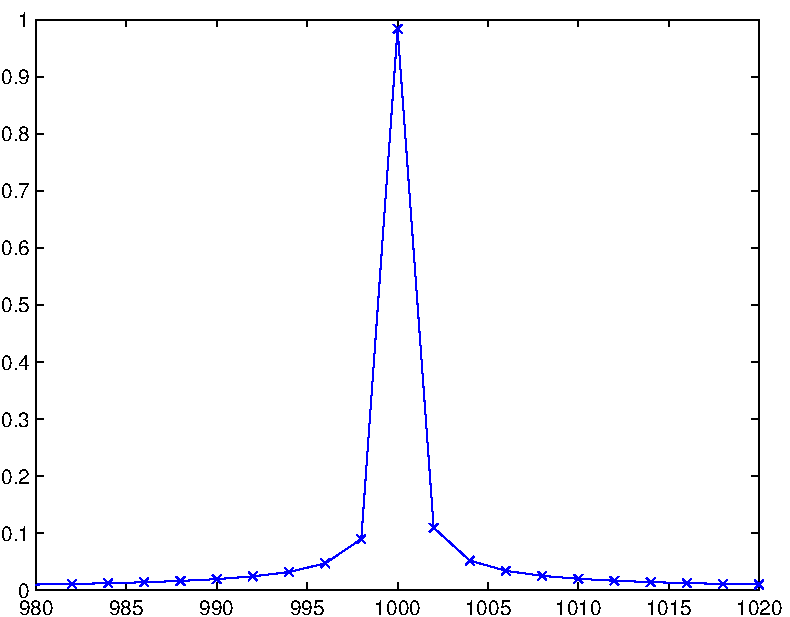
\includegraphics[width=0.7\textwidth]{qwtb_examples_published/qwtb_example_1_01.pdf}
\end{center}
\begin{par}
One can see it is not a coherent measurement. Therefore to get 'unknown' amplitude and frequency of the signal algorithm \lstinline{PSFE} can be used:
\end{par} \vspace{1em}
\begin{lstlisting}[style=mcode]
DO = qwtb('PSFE', DI);
f = DO.f.v
A = DO.A.v
\end{lstlisting}

        \begin{lstlisting}[style=output]
QWTB: no uncertainty calculation

f =

   1.0000e+03


A =

    1.0000

\end{lstlisting} \color{black}
    

\subsubsection*{Uncertainties}

\begin{par}
Uncertainties are added to the \lstinline{t} (time stamps) and \lstinline{y} (sampled data) structures.
\end{par} \vspace{1em}
\begin{lstlisting}[style=mcode]
DI.t.u = zeros(size(DI.t.v)) + 1e-5;
DI.y.u = zeros(size(DI.y.v)) + 1e-4;
\end{lstlisting}
\begin{par}
Calculations settings is created with Monte Carlo uncertainty calculation method, 1000 repeats and singlecore calculation.
\end{par} \vspace{1em}
\begin{lstlisting}[style=mcode]
CS.unc = 'mcm';
CS.mcm.repeats = 1000;
CS.mcm.method = 'singlecore';
\end{lstlisting}
\begin{par}
Run PSFE algorithm on input data \lstinline{DI} and with calculattion settings \lstinline{CS}.
\end{par} \vspace{1em}
\begin{lstlisting}[style=mcode]
DO = qwtb('PSFE',DI,CS);
\end{lstlisting}

        \begin{lstlisting}[style=output]
QWTB: default correlation matrix generated for quantity `t`
QWTB: quantity t was randomized by QWTB
QWTB: default correlation matrix generated for quantity `y`
QWTB: quantity y was randomized by QWTB
QWTB: general mcm uncertainty calculation
\end{lstlisting} \color{black}
    \begin{par}
Result is displayed as a histogram of calculated frequency.
\end{par} \vspace{1em}
\begin{lstlisting}[style=mcode]
figure; hist(DO.f.r,50);
\end{lstlisting}

\begin{center}
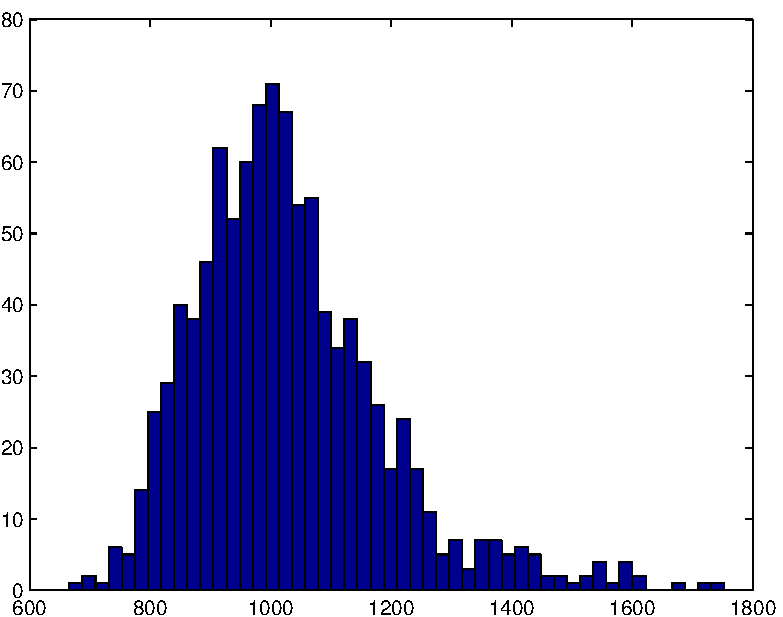
\includegraphics[width=0.7\textwidth]{qwtb_examples_published/qwtb_example_1_02.pdf}
\end{center}
\begin{par}
One can see the histogram is not Gaussian function. To get correct uncertainties, a shortest covariant interval has to be used.
\end{par} \vspace{1em}



%%% \end{document}
    


\chapter{Long example of QWTB use} %<<<1 ----------------------------------

% This LaTeX was auto-generated from an M-file by MATLAB.
% To make changes, update the M-file and republish this document.

%%% \documentclass{article}
%%% \usepackage{graphicx}
%%% \usepackage{color}

%%% \sloppy
%%% \definecolor{lightgray}{gray}{0.5}
\setlength{\parindent}{0pt}

%%% \begin{document}

    
    
\subsection*{Example of the QWTB use}

\begin{par}
Data are simulated, QWTB is used with different algorithms.
\end{par} \vspace{1em}

\subsubsection*{Contents}

\begin{itemize}
\setlength{\itemsep}{-1ex}
   \item Generate ideal data
   \item Apply three algorithms
   \item Compare results for ideal signal
   \item Noisy signal
   \item Compare results for noisy signal
   \item Non-coherent signal
   \item Compare results for non-coherent signal
   \item Harmonically distorted signal.
   \item Compare results for harmonically distorted signal.
   \item Harmonically distorted, noisy, non-coherent signal.
   \item Compare results for harmonically distorted, noisy, non-coherent signal.
\end{itemize}


\subsubsection*{Generate ideal data}

\begin{par}
Sample data are generated, representing 1 second of sine waveform of nominal frequency \lstinline{fnom} 1000 Hz, nominal amplitude \lstinline{Anom} 1 V and nominal phase \lstinline{phnom} 1 rad. Data are sampled at sampling frequency \lstinline{fsnom} 10 kHz, perfectly synchronized, no noise.
\end{par} \vspace{1em}
\begin{lstlisting}[style=mcode]
Anom = 1; fnom = 1000; phnom = 1; fsnom = 10e4;
timestamps = [0:1/fsnom:0.1-1/fsnom];
ideal_wave = Anom*sin(2*pi*fnom*timestamps + phnom);
\end{lstlisting}
\begin{par}
To use QWTB, data are put into two quantities: \lstinline{t} and \lstinline{y}. Both quantities are put into data in structure \lstinline{DI}.
\end{par} \vspace{1em}
\begin{lstlisting}[style=mcode]
DI = [];
DI.t.v = timestamps;
DI.y.v = ideal_wave;
\end{lstlisting}


\subsubsection*{Apply three algorithms}

\begin{par}
QWTB will be used to apply three algorithms to determine frequency and amplitude: \lstinline{SP-FFT}, \lstinline{PSFE} and \lstinline{FPNLSF}. Results are in data out structure \lstinline{DOxxx}. Algorithm \lstinline{FPNLSF} requires an estimate, select it to 0.1\% different from nominal frequency. \lstinline{SP-FFT} requires sampling frequency.
\end{par} \vspace{1em}
\begin{lstlisting}[style=mcode]
DI.fest.v = fnom.*1.001;
DI.fs.v = fsnom;
DOspfft = qwtb('SP-FFT', DI);
DOpsfe = qwtb('PSFE', DI);
DOfpnlsf = qwtb('FPNLSF', DI);
\end{lstlisting}

        \begin{lstlisting}[style=output]
QWTB: no uncertainty calculation
QWTB: no uncertainty calculation
QWTB: PSFE wrapper: sampling time was calculated from sampling frequency
QWTB: no uncertainty calculation
Fitting started

Local minimum found.

Optimization completed because the size of the gradient is less than
the default value of the function tolerance.



Fitting finished
\end{lstlisting} \color{black}
    

\subsubsection*{Compare results for ideal signal}

\begin{par}
Calculate relative errors in ppm for all algorithm to know which one is best. \lstinline{SP-FFT} returns whole spectrum, so only the largest amplitude peak is interesting. One can see for the ideal case all errors are very small.
\end{par} \vspace{1em}
\begin{lstlisting}[style=mcode]
disp('SP-FFT errors (ppm):')
[tmp, ind] = max(DOspfft.A.v);
ferr  = (DOspfft.f.v(ind) - fnom)/fnom .* 1e6
Aerr  = (DOspfft.A.v(ind) - Anom)/Anom .* 1e6
pherr = (DOspfft.ph.v(ind) - phnom)/phnom .* 1e6

disp('PSFE errors (ppm):')
ferr  = (DOpsfe.f.v - fnom)/fnom .* 1e6
Aerr  = (DOpsfe.A.v - Anom)/Anom .* 1e6
pherr = (DOpsfe.ph.v - phnom)/phnom .* 1e6

disp('FPNLSF errors (ppm):')
ferr  = (DOfpnlsf.f.v - fnom)/fnom .* 1e6
Aerr  = (DOfpnlsf.A.v - Anom)/Anom .* 1e6
pherr = (DOfpnlsf.ph.v - phnom)/phnom .* 1e6
\end{lstlisting}

        \begin{lstlisting}[style=output]
SP-FFT errors (ppm):

ferr =

     0


Aerr =

     0


pherr =

  -4.2920e+05

PSFE errors (ppm):

ferr =

  -2.2737e-10


Aerr =

   4.8850e-09


pherr =

   2.3093e-08

FPNLSF errors (ppm):

ferr =

  -3.4106e-10


Aerr =

  -4.0512e-07


pherr =

   1.8208e-08

\end{lstlisting} \color{black}
    

\subsubsection*{Noisy signal}

\begin{par}
To simulate real measurement, noise is added with normal distribution and standard deviation \lstinline{sigma} of 100 microvolt. Algorithms are again applied.
\end{par} \vspace{1em}
\begin{lstlisting}[style=mcode]
sigma = 100e-6;
DI.y.v = ideal_wave + 100e-6.*randn(size(ideal_wave));
DOspfft = qwtb('SP-FFT', DI);
DOpsfe = qwtb('PSFE', DI);
DOfpnlsf = qwtb('FPNLSF', DI);
\end{lstlisting}

        \begin{lstlisting}[style=output]
QWTB: no uncertainty calculation
QWTB: no uncertainty calculation
QWTB: PSFE wrapper: sampling time was calculated from sampling frequency
QWTB: no uncertainty calculation
Fitting started

Local minimum found.

Optimization completed because the size of the gradient is less than
the default value of the function tolerance.



Fitting finished
\end{lstlisting} \color{black}
    

\subsubsection*{Compare results for noisy signal}

\begin{par}
Again relative errors are compared. One can see amplitude and phase errors increased to several ppm, however frequency is still determined quite good by all three algorithms. FFT is not affected by noise at all.
\end{par} \vspace{1em}
\begin{lstlisting}[style=mcode]
disp('SP-FFT errors (ppm):')
[tmp, ind] = max(DOspfft.A.v);
ferr  = (DOspfft.f.v(ind) - fnom)/fnom .* 1e6
Aerr  = (DOspfft.A.v(ind) - Anom)/Anom .* 1e6
pherr = (DOspfft.ph.v(ind) - phnom)/phnom .* 1e6

disp('PSFE errors:')
ferr  = (DOpsfe.f.v - fnom)/fnom .* 1e6
Aerr  = (DOpsfe.A.v - Anom)/Anom .* 1e6
pherr = (DOpsfe.ph.v - phnom)/phnom .* 1e6

disp('FPNLSF errors:')
ferr  = (DOfpnlsf.f.v - fnom)/fnom .* 1e6
Aerr  = (DOfpnlsf.A.v - Anom)/Anom .* 1e6
pherr = (DOfpnlsf.ph.v - phnom)/phnom .* 1e6
\end{lstlisting}

        \begin{lstlisting}[style=output]
SP-FFT errors (ppm):

ferr =

     0


Aerr =

   -0.6603


pherr =

  -4.2920e+05

PSFE errors:

ferr =

    0.0010


Aerr =

   -0.6318


pherr =

   -1.0933

FPNLSF errors:

ferr =

   -0.0011


Aerr =

   -0.6601


pherr =

   -0.3809

\end{lstlisting} \color{black}
    

\subsubsection*{Non-coherent signal}

\begin{par}
In real measurement coherent measurement does not exist. So in next test the frequency of the signal differs by 20 ppm:
\end{par} \vspace{1em}
\begin{lstlisting}[style=mcode]
fnc = fnom*(1 + 20e-6);
noncoh_wave = Anom*sin(2*pi*fnc*timestamps + phnom);
DI.y.v = noncoh_wave;
DOspfft = qwtb('SP-FFT', DI);
DOpsfe = qwtb('PSFE', DI);
DOfpnlsf = qwtb('FPNLSF', DI);
\end{lstlisting}

        \begin{lstlisting}[style=output]
QWTB: no uncertainty calculation
QWTB: no uncertainty calculation
QWTB: PSFE wrapper: sampling time was calculated from sampling frequency
QWTB: no uncertainty calculation
Fitting started

Local minimum found.

Optimization completed because the size of the gradient is less than
the default value of the function tolerance.



Fitting finished
\end{lstlisting} \color{black}
    

\subsubsection*{Compare results for non-coherent signal}

\begin{par}
Comparison of relative errors. Results of \lstinline{PSFE} or \lstinline{FPNLSF} are correct, however FFT is affected by non-coherent signal considerably.
\end{par} \vspace{1em}
\begin{lstlisting}[style=mcode]
disp('SP-FFT errors (ppm):')
[tmp, ind] = max(DOspfft.A.v);
ferr  = (DOspfft.f.v(ind) - fnc)/fnc .* 1e6
Aerr  = (DOspfft.A.v(ind) - Anom)/Anom .* 1e6
pherr = (DOspfft.ph.v(ind) - phnom)/phnom .* 1e6

disp('PSFE errors:')
ferr  = (DOpsfe.f.v - fnc)/fnc .* 1e6
Aerr  = (DOpsfe.A.v - Anom)/Anom .* 1e6
pherr = (DOpsfe.ph.v - phnom)/phnom .* 1e6

disp('FPNLSF errors:')
ferr  = (DOfpnlsf.f.v - fnc)/fnc .* 1e6
Aerr  = (DOfpnlsf.A.v - Anom)/Anom .* 1e6
pherr = (DOfpnlsf.ph.v - phnom)/phnom .* 1e6
\end{lstlisting}

        \begin{lstlisting}[style=output]
SP-FFT errors (ppm):

ferr =

  -19.9996


Aerr =

   -2.8780


pherr =

  -4.3550e+05

PSFE errors:

ferr =

  -1.1368e-10


Aerr =

   3.8924e-07


pherr =

   3.3073e-04

FPNLSF errors:

ferr =

  -1.1368e-10


Aerr =

  -3.2940e-07


pherr =

   2.6867e-08

\end{lstlisting} \color{black}
    

\subsubsection*{Harmonically distorted signal.}

\begin{par}
In other cases a harmonic distortion can appear. Suppose a signal with second order harmonic of 10\% amplitude as the main signal.
\end{par} \vspace{1em}
\begin{lstlisting}[style=mcode]
hadist_wave = Anom*sin(2*pi*fnom*timestamps + phnom) + 0.1*Anom*sin(2*pi*fnom*2*timestamps + 2);
DI.y.v = hadist_wave;
DOspfft = qwtb('SP-FFT', DI);
DOpsfe = qwtb('PSFE', DI);
DOfpnlsf = qwtb('FPNLSF', DI);
\end{lstlisting}

        \begin{lstlisting}[style=output]
QWTB: no uncertainty calculation
QWTB: no uncertainty calculation
QWTB: PSFE wrapper: sampling time was calculated from sampling frequency
QWTB: no uncertainty calculation
Fitting started

Local minimum found.

Optimization completed because the size of the gradient is less than
the default value of the function tolerance.



Fitting finished
\end{lstlisting} \color{black}
    

\subsubsection*{Compare results for harmonically distorted signal.}

\begin{par}
Comparison of relative errors. \lstinline{SP-FFT} or \lstinline{PSFE} are not affected by harmonic distortion, however \lstinline{FPNLSF} is thus is not suitable for such signal.
\end{par} \vspace{1em}
\begin{lstlisting}[style=mcode]
disp('SP-FFT errors (ppm):')
[tmp, ind] = max(DOspfft.A.v);
ferr  = (DOspfft.f.v(ind) - fnom)/fnom .* 1e6
Aerr  = (DOspfft.A.v(ind) - Anom)/Anom .* 1e6
pherr = (DOspfft.ph.v(ind) - phnom)/phnom .* 1e6

disp('PSFE errors:')
ferr  = (DOpsfe.f.v - fnom)/fnom .* 1e6
Aerr  = (DOpsfe.A.v - Anom)/Anom .* 1e6
pherr = (DOpsfe.ph.v - phnom)/phnom .* 1e6

disp('FPNLSF errors:')
ferr  = (DOfpnlsf.f.v - fnom)/fnom .* 1e6
Aerr  = (DOfpnlsf.A.v - Anom)/Anom .* 1e6
pherr = (DOfpnlsf.ph.v - phnom)/phnom .* 1e6
\end{lstlisting}

        \begin{lstlisting}[style=output]
SP-FFT errors (ppm):

ferr =

     0


Aerr =

     0


pherr =

  -4.2920e+05

PSFE errors:

ferr =

  -2.2737e-10


Aerr =

   6.7212e-04


pherr =

    0.5311

FPNLSF errors:

ferr =

   -0.7356


Aerr =

    0.1407


pherr =

  231.4553

\end{lstlisting} \color{black}
    

\subsubsection*{Harmonically distorted, noisy, non-coherent signal.}

\begin{par}
In final test all distortions are put in a waveform and results are compared.
\end{par} \vspace{1em}
\begin{lstlisting}[style=mcode]
err_wave = Anom*sin(2*pi*fnc*timestamps + phnom) + 0.1*Anom*sin(2*pi*fnc*2*timestamps + 2) + 100e-6.*randn(size(ideal_wave));
DI.y.v = err_wave;
DOspfft = qwtb('SP-FFT', DI);
DOpsfe = qwtb('PSFE', DI);
DOfpnlsf = qwtb('FPNLSF', DI);
\end{lstlisting}

        \begin{lstlisting}[style=output]
QWTB: no uncertainty calculation
QWTB: no uncertainty calculation
QWTB: PSFE wrapper: sampling time was calculated from sampling frequency
QWTB: no uncertainty calculation
Fitting started

Local minimum found.

Optimization completed because the size of the gradient is less than
the default value of the function tolerance.



Fitting finished
\end{lstlisting} \color{black}
    

\subsubsection*{Compare results for harmonically distorted, noisy, non-coherent signal.}

\begin{lstlisting}[style=mcode]
disp('SP-FFT errors (ppm):')
[tmp, ind] = max(DOspfft.A.v);
ferr  = (DOspfft.f.v(ind) - fnc)/fnc .* 1e6
Aerr  = (DOspfft.A.v(ind) - Anom)/Anom .* 1e6
pherr = (DOspfft.ph.v(ind) - phnom)/phnom .* 1e6

disp('PSFE errors:')
ferr  = (DOpsfe.f.v - fnc)/fnc .* 1e6
Aerr  = (DOpsfe.A.v - Anom)/Anom .* 1e6
pherr = (DOpsfe.ph.v - phnom)/phnom .* 1e6

disp('FPNLSF errors:')
ferr  = (DOfpnlsf.f.v - fnc)/fnc .* 1e6
Aerr  = (DOfpnlsf.A.v - Anom)/Anom .* 1e6
pherr = (DOfpnlsf.ph.v - phnom)/phnom .* 1e6
\end{lstlisting}

        \begin{lstlisting}[style=output]
SP-FFT errors (ppm):

ferr =

  -19.9996


Aerr =

    1.1501


pherr =

  -4.3550e+05

PSFE errors:

ferr =

   -0.0072


Aerr =

    4.1189


pherr =

    4.6464

FPNLSF errors:

ferr =

   -0.7241


Aerr =

    3.6943


pherr =

  229.3720

\end{lstlisting} \color{black}
    


%%% \end{document}
    


\end{document}

% vim settings: vim:foldmarker=%<<<,%>>> fdm=marker fen
